\chapter{Conceitos Básicos}
\label{cap:2}

Reproduzir uma sequência de imagens similares para criar uma ilusão de movimento é uma prática existente desde o final do século XIX, tal como consta em \cite{bib:sciam_firstmotion}, publicação científica mais antiga sobre o tema. Cada nova imagem (denominada quadro) é sutilmente diferente da anterior, sendo que esta sutileza cresce à medida que aumenta a velocidade de captação entre essas imagens. Ao compararmos dois quadros próximos, constatamos que a diferença entre eles tende a ser mínima, ainda mais quando se tratam de vídeos com alta taxa de transição de imagem para cada unidade de tempo considerado, normalmente um segundo. 

Em um vídeo digital, cada quadro é composto por partes menores, denominadas pixels. Sendo o pixel o menor elemento de uma imagem digital, este é, por sua vez, o elemento que informa a cor de cada ponto daquela imagem. Os pixels representam valores em um padrão de cores. Normalmente, três valores inteiros, chamados de amostras, são utilizados para representar a intensidade de vermelho, verde e azul, no caso do sistema de cores RGB, ou de luminância, crominância azul e crominância vermelha, no caso do sistema de cores YCbCr \cite{bib:sistema_cores}.

No caso de vídeos armazenados digitalmente, observamos que a maior parte de um vídeo sem compressão conterá dados redundantes. Para possibilitar a redução desses dados, a codificação de vídeos deve ser especializada em identificar e explorar três tipos de redundância, conforme afirma \cite{bib:tese_agostini_2007}. As redundâncias que o codificador de vídeo busca identificar são: 

\begin{enumerate}[a)]
    \item \textbf{Redundância Temporal}: manifesta-se através da existência de dados repetidos entre dois quadros vizinhos;

    \item \textbf{Redundância Espacial}: manifesta-se através da existência de dados repetidos dentro de um mesmo quadro;

    \item \textbf{Redundância Entrópica}: manifesta-se através da distribuição dos símbolos, ou probabilidade de ocorrência de símbolos, em um vídeo.
\end{enumerate}

Apesar de haver diversos codificadores de vídeo desenvolvidos para determinados fins, em geral os formatos e padrões lançados nas últimas duas décadas são classificados como formatos de codificação de vídeo híbrida \cite{bib:richardson_2002}, ou seja, combina diversas técnicas de codificação visando alcançar o melhor resultado possível em termos de eficiência de compressão. Essa codificação híbrida é baseada em blocos, onde cada bloco é composto por um conjunto de pixels, também denominados de amostras. Eles recebem essa classificação por explorarem diversos tipos de redundâncias a fim de atingir altas taxas de compressão \cite{bib:tese_agostini_2007}. Apesar dos formatos possuírem diferenças pontuais, é possível resumir o fluxo de execução de um codificador de vídeo híbrido baseado em blocos conforme a Figura \ref{fig:2}. Todas essas etapas são executadas ou associadas ao nível de bloco e, apesar dos codificadores modernos já serem mais complexos do que o explicado aqui, o resumo dessas etapas segue conforme listado abaixo:

\begin{figure}
    \centering
    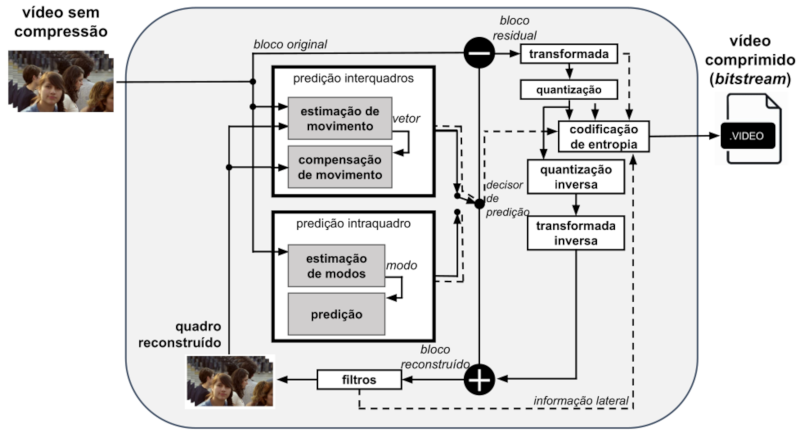
\includegraphics[width=\textwidth]{FIGURES/fig_2.png}
    \caption{Representação em alto nível de um codificador de vídeo híbrido. Fonte: Elaborada pelo autor.}
    \label{fig:2}
\end{figure}


\begin{itemize}
    \item \textbf{Predição Intraquadro}: responsável por predizer os valores das amostras do bloco que se está processando apenas utilizando informações do próprio quadro de origem do bloco, de forma a reduzir a redundância espacial. Para tanto, são usados modos de predição que indicam ao codificador/decodificador em qual direção está a amostra que contém o valor que deve ser copiado. O primeiro quadro de cada vídeo codificado, atualmente, é somente processado por esse tipo de predição, já que não há dependência de dados anteriores para sua funcionalidade. Além disso, esse tipo de quadro exclusivo de predição intraquadro também é utilizado, por exemplo, para sincronização durante transmissões ao vivo;

    \item \textbf{Predição Interquadros}: responsável por reduzir a redundância temporal, é uma predição dependente de quadros vizinhos para ser executada. Seu funcionamento consiste em varrer blocos de amostras do quadro de referência (localizados anteriormente ou posteriormente ao quadro atual) buscando um bloco que seja igual ou similar ao bloco de amostras sob codificação no momento. O resultado dessa predição é um vetor de movimento que aponta o deslocamento que deve ser realizado, a partir da posição do bloco sob codificação, para encontrar o bloco de referência;

    \item \textbf{Transformada}: da subtração do bloco predito com o bloco original, obtém-se um bloco residual. Este bloco é importante pois define diferença entre os blocos original e predito, ou seja, define o erro de predição (seja intraquadro ou interquadros). Entretanto, ele representa informações no domínio espacial, no qual as amostras ainda estão correlacionados entre si, o que leva a um baixo desempenho da codificação de entropia. Para possibilitar uma decorrelação da informação residual e concentrá-la em um pequeno número de coeficientes, os blocos residuais são submetidos a um processo de transformação do domínio de representação, passando-os do domínio espacial para o domínio de frequências;

    \item \textbf{Quantização}: com os dados representados no domínio das frequências e considerando o funcionamento do sistema visual humano, é possível atenuar, ou mesmo eliminar, frequências mais elevadas que pouco contribuem para a formação da imagem pelo olho humano. Esse processo de atenuação/eliminação é feito nesta etapa de codificação, na qual ocorre a aplicação de um parâmetro de quantização sobre os coeficientes transformados, gerando um bloco quantizado. Até esta etapa, ao menos para os formatos publicados nas últimas duas décadas, todos os processos realizados são totalmente reversíveis, no entanto, após a aplicação da quantização, informações são irreversivelmente descartadas e, portanto, perdas na qualidade da imagem são geradas;

    \item \textbf{Codificação de Entropia}: responsável pela compressão propriamente dita. A codificação de entropia processa os dados transformados e quantizados, assim como as informações laterais (modos decididos, tamanhos de blocos, etc.). Todos os estágios de codificação servem para tornar este estágio mais eficiente, pois quanto menores são os resíduos e, consequentemente, mais concentrados são os coeficientes transformados e quantizados, maior é a taxa de compressão obtida pela codificação de entropia. Ao final desta etapa, é gerado um \textit{bitstream} compatível com o formato de vídeo utilizado durante a codificação;

    \item \textbf{Filtros}: responsável por reduzir, ou mesmo eliminar, artefatos de compressão causados pela etapa de quantização. Há diversos artefatos de compressão, apresentados em \citet{bib:quantization_artifacts}, como o efeito de bloco, de borramento, entre outros. A aplicação desta etapa de codificação implica na suavização das diferenças entre o vídeo codificado com o vídeo original.

\end{itemize}

Além desses seis estágios de codificação, dentro do próprio codificador inclui-se parte do decodificador, com a quantização inversa e a transformada inversa, com o objetivo de reconstruir o quadro a fim de ser utilizado como referência pelos estágios de predição. Isso serve para garantir que as referências de predições sejam as mesmas no codificador e no decodificador. Apesar de os seis estágios de codificação de vídeo apresentados acima serem similares entre os codificadores de vídeo da atualidade, eles se diferem quanto à forma de executar as operações ou quanto às variações de decisões disponíveis para serem escolhidas. Por exemplo, enquanto o codificador H.264/AVC possui nove modos diferentes de predição intraquadro, o H.266/VVC dispõe 72 modos distintos \cite{bib:vvc_intra_modes}, provendo uma maior flexibilidade para que o codificador possa se adaptar a características específicas do vídeo que está sendo codificado. Outro exemplo é a quantidade de tamanhos de blocos disponíveis no formato VP9, que é de 13, enquanto seu sucessor direto, o AV1, dispõe de 22 \cite{bib:av1_overview_2021}. Com isso, fica compreensível o elevado custo computacional de codificadores modernos em relação aos lançados anteriormente, pois, além de aumentar o número de opções disponíveis para escolha em cada etapa de codificação, o próprio processo de escolher uma dessas opções é deveras custoso, computacionalmente falando. Para finalizar esta breve explicação do funcionamento de um codificador híbrido, destaca-se esse processo decisório que avalia as diversas variações disponíveis em cada um dos estágios citados, indicando qual deve ser utilizado. Cada software de codificação implementa um algoritmo próprio para identificar a melhor decisão a ser tomada, e esses algoritmos são evoluções do trabalho de \citet{bib:rdo_sullivan}, tipificados como algoritmos de otimização da taxa-distorção (do inglês \textit{Rate-Distortion Optimization}, RDO).

Além disso, é relevante para o escopo desta tese discutir o percentual de representatividade de informação que cada tamanho de bloco apresenta em relação às diversas resoluções de vídeo disponíveis. Quanto menor o tamanho N$\times$N de um bloco, menor é a proporção de dados que este apresenta em relação ao quadro; da mesma forma, quanto maior a resolução de um vídeo, menor é a proporção de dados que um bloco de tamanho N$\times$N apresenta em relação ao quadro. Por exemplo, considerando um bloco de tamanho 128$\times$128, ora esse bloco pode representar um rosto inteiro (em vídeos de baixa resolução), ora apenas um pequeno detalhe do rosto (em vídeos de alta resolução). 

A Tabela \ref{tab:I} apresenta a relação entre os tamanhos quadráticos de blocos comuns entre os formatos de codificação de vídeo atuais e seu percentual de representatividade de informação para diferentes resoluções de vídeo. Com essa tabela, é possível perceber que a predição dos pixels de um bloco de tamanho 128$\times$128 em um vídeo de resolução 176$\times$144 (também identificada como QCIF) é uma tarefa difícil, tornando escassas as probabilidades de que uma predição a ser realizada neste bloco retorne bons resultados. Neste caso, o bloco representa 64\% do quadro todo e uma má predição no bloco afeta 64\% da área visível para o usuário. Por outro lado, esse mesmo tamanho de bloco representa apenas 0,79\% de um quadro em resolução 1920$\times$1080 (HD 1080). Logo, menor será a probabilidade de más predições ocasionarem impacto significativo na qualidade da imagem ou na eficiência de codificação.

\begin{table}
\begin{center}
\caption{Proporção (em porcentagem) de representação de informação de blocos de diferentes tamanhos em diferentes resoluções de vídeo.}
\label{tab:I}
\footnotesize

\begin{tblr}{
    colspec = {p{2.3cm}|rrrrrr},
    hlines,
    row{even} = {gray9}
}
\hline
\SetCell[r=2]{c}\textbf{Resolução do Vídeo} & \SetCell[c=6]{c}\textbf{Tamanho do Bloco} \\
 & \SetCell[r=1]{c}4$\times$4 & \SetCell[r=1]{c}8$\times$8 & \SetCell[r=1]{c}16$\times$16 & \SetCell[r=1]{c}32$\times$32 & \SetCell[r=1]{c}64$\times$64 & \SetCell[r=1]{c}128$\times$128 \\
 
\SetCell[r=1]{c}176$\times$144 & 0,06313 & 0,25253 & 1,01010 & 4,04040 & 16,16162 & 64,64646 \\
\SetCell[r=1]{c}426$\times$240 & 0,01565 & 0,06260 & 0,25039 & 1,00156 & 4,00626 & 16,02504 \\
\SetCell[r=1]{c}640$\times$360 & 0,00694 & 0,02778 & 0,11111 & 0,44444 & 1,77778 & 7,11111 \\
\SetCell[r=1]{c}832$\times$480 & 0,00401 & 0,01603 & 0,06410 & 0,25641 & 1,02564 & 4,10256 \\
\SetCell[r=1]{c}1280$\times$720  & 0,00174 & 0,00694 & 0,02778 & 0,11111 & 0,44444 & 1,77778 \\
\SetCell[r=1]{c}1920$\times$1080 & 0,00077 & 0,00309 & 0,01235 & 0,04938 & 0,19753 & 0,79012 \\
\SetCell[r=1]{c}4096$\times$2160 & 0,00018 & 0,00072 & 0,00289 & 0,01157 & 0,04630 & 0,18519 \\
\SetCell[r=1]{c}7680$\times$4320 & 0,00005 & 0,00019 & 0,00077 & 0,00309 & 0,01235 & 0,04938 \\
\hline
\end{tblr}
\end{center}
\end{table}


\section{Transcodificação de Vídeo}
\label{cap:2.1}

A modificação do \textit{bitstream} de vídeo codificado é uma prática comum na indústria e visa sanar as mais diversas necessidades. Uma delas é a migração de vídeos codificados com tecnologias mais antigas para tecnologias mais recentes e mais eficientes em termos de compressão de dados. Outra é permitir que uma transmissão seja compatível com os mais diversos reprodutores de vídeo disponíveis no mercado, o que só é possível se o transmissor do vídeo disponibilizar \textit{bitstream}s para os mais diversos formatos. Essas e tantas outras necessidades são satisfeitas através do uso de um transcodificador de vídeo. O funcionamento básico da transcodificação de vídeo, conforme ilustrado na Figura \ref{fig:3}, pode ser resumido em um processo em cascata no qual um vídeo codificado com a tecnologia antiga (OLD) é decodificado e recodificado com uma tecnologia nova (NEW). Esse modelo geral de transcodificação de vídeo, também denominado como transcodificador em cascata, ou típico, ou ainda original (inclusive, este último será utilizado no decorrer da tese), não é exclusivo de formatos digitais, já sendo utilizado desde o advento de transmissão comercial de programas de televisão, no qual a migração de sinais analógicos de vídeos já era comum. Isso pode ser visto em \cite{bib:transcoding67}, quem propôs uma solução em hardware capaz de modificar o sinal de vídeos originários da Europa Ocidental para se adequarem aos televisores norte-americanos, já que a frequência eletromagnética e a organização das linhas de raios catódicos dos televisores eram divergentes entre as duas regiões.

\begin{figure}
    \centering
    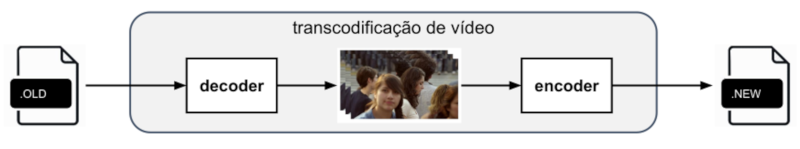
\includegraphics[width=\textwidth]{FIGURES/fig_3.png}
    \caption{Visão em alto nível de um transcodificador de vídeo original. Fonte: Elaborada pelo autor.}
    \label{fig:3}
\end{figure}

Atualmente, na era das tecnologias digitais, há dois tipos fundamentais de transcodificadores: heterogêneos e homogêneos. Eles são facilmente identificados ao se observar quais são os formatos utilizados em uma transcodificação: caso OLD e NEW sejam iguais, trata-se de uma transcodificação homogênea; caso contrário, uma transcodificação heterogênea. Apesar da transcodificação homogênea não envolver troca no formato de codificação, é muito utilizada pela indústria de vídeos, de modo a atingir algum objetivo particular, como a redução da taxa de bits por segundo, redução da resolução, adaptação do \textit{bitstream} para diferentes configurações temporais, inserção de marca d’água, etc. Em \citet{bib:modosTranscodificacao}, o autor identificou diversas utilizações de um transcodificador de vídeo, vide Figura \ref{fig:4}.

\begin{figure}
    \centering
    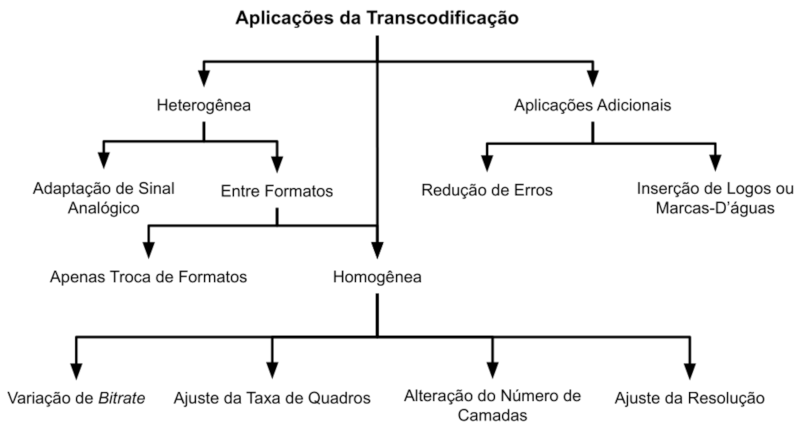
\includegraphics[width=\textwidth]{FIGURES/fig_4.png}
    \caption{Classificação de transcodificadores de vídeo. Fonte: Elaborada pelo autor com base em \citet{bib:modosTranscodificacao}.}
    \label{fig:4}
\end{figure}

Na literatura científica, a transcodificação homogênea é apresentada, principalmente, como solução para a redução da taxa de bits do vídeo (também identificado como \textit{transrating}), como no trabalho de \citet{bib:nam_2006}, mas também para a redução da resolução do vídeo, como em \citet{bib:nguyen_2015}. Esta última modalidade, que pode ser identificada como \textit{downscaling}, visa adequar a resolução original do vídeo para os mais diversos meios de reprodução que o usuário possa utilizar, já que, quando a resolução do vídeo é reduzida, a taxa de bits também o é. A preocupação com a redução do tamanho do \textit{bitstream} de forma a se adequar à largura de banda na transmissão de vídeo pode ser observada desde os princípios da internet, como pode ser visto nos trabalhos de \citet{bib:shen_1997} e \citet{bib:swann_1996}, que propuseram soluções de transcodificação para adequar o \textit{bitstream} a diferentes meios de transmissão de dados, de forma a apresentar o menor erro possível na transmissão do vídeo e manter a experiência do usuário relativamente adequada. Como na transcodificação homogênea o software codificador opera com o mesmo formato de codificação que o decodificador, a diferença entre as versões do \textit{bitstream} está em particularidades da codificação, isto é, nas configurações utilizadas.

Já a transcodificação heterogênea visa de fato a mudança no formato de codificação de vídeo usado. Uma das principais razões para se aplicar esse tipo de transcodificação é permitir a compatibilidade de um vídeo com diferentes sistemas de reprodução. Em outras palavras, um vídeo codificado com tecnologias recentes que precisa ser reproduzido em sistemas antigos (\textit{backward compatibility}) ou um vídeo codificado com tecnologias antigas que precisa ser atualizado para reprodução em sistemas mais recentes (\textit{forward compatibility}). Outros motivos, como a existência de políticas de royalties associadas à reprodução de vídeos em certos formatos, também podem motivar a conversão entre formatos. A existência de múltiplos sistemas de reprodução de vídeo no mundo real é também uma razão para que empresas necessitem manter seus vídeos em mais de um formato de codificação, como é o caso do YouTube, que oferece suporte simultaneamente aos formatos H.264, VP9 e AV1 \cite{bib:bitmovin_ott_report_2020} \cite{bib:5to9google}.

Por fim, como mostra a Figura \ref{fig:4}, também há uma categoria de transcodificação para aplicações adicionais, que não busca realizar uma modificação do \textit{bitstream} propriamente dita, mas apenas incluir nele funcionalidades novas, como inserção de marca-d'água, legendas (embutidas ou não), novas opções de idioma, etc. Normalmente esse tipo de transcodificação não é comum na literatura científica, mas pode-se citar o trabalho de \citet{bib:watermark}, que visa remover marcas-d’água existentes em vídeos.

A correta categorização da transcodificação é útil em duas situações específicas: saber quais parâmetros da codificação devem ser configurados e quais informações são particularmente importantes para serem consideradas durante uma transcodificação de vídeo acelerada. Nesta tese, destacamos principalmente os trabalhos voltados para transcodificações heterogêneas, pois os custos computacionais de execução de um codificador e um decodificador se dão em escalas diferentes. O codificador deve considerar todas as opções disponíveis no formato de codificação a fim de encontrar a melhor combinação de decisões para cada região do vídeo, gerando assim um \textit{bitstream} com a maior eficiência de codificação possível. O decodificador, por sua vez, precisa apenas reverter o \textit{bitstream} em arquivo de vídeo. Logo, havendo a possibilidade de reduzir o custo computacional ao executar o codificador, ela deve ser aproveitada.

Observa-se o emprego de quatro estratégias para realizar a transcodificação rápida:

\begin{itemize}
    \item A partir do reaproveitamento de informações provenientes exclusivamente do decodificador, com soluções baseadas em heurísticas;
    
    \item A partir do reaproveitamento de informações provenientes tanto do decodificador como do codificador, com soluções baseadas em heurísticas;

    \item A partir do reaproveitamento de informações provenientes exclusivamente do decodificador, com soluções baseadas em modelos preditivos treinados por aprendizado de máquina;

    \item A partir do reaproveitamento de informações provenientes tanto do decodificador como do codificador, com soluções baseadas em modelos preditivos treinados por aprendizado de máquina.
\end{itemize}

Apesar de todas as opções acima serem representáveis pela Figura \ref{fig:5}, a origem dos reaproveitamentos na figura leva em conta apenas informações extraídas do decodificador. Todavia, também é possível o reaproveitamento de informações provenientes do próprio codificador.

\begin{figure}
    \centering
    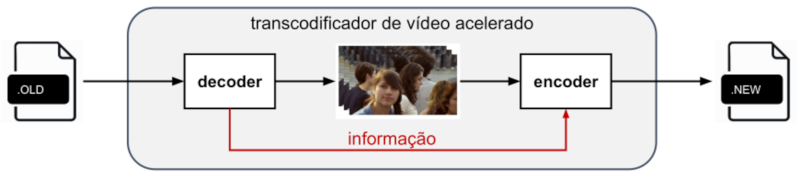
\includegraphics[width=\textwidth]{FIGURES/fig_5.png}
    \caption{Representação em alto nível de uma transcodificação rápida de vídeo. Fonte: Elaborada pelo autor.}
    \label{fig:5}
\end{figure}

Independentemente da classificação de transcodificador rápido que se faz uso, existe, em todas elas, a possibilidade de obter os dados provenientes do processo de decodificação, sendo possível transformá-los em conhecimento sobre o vídeo que será codificado. Portanto, esse conhecimento deve ser utilizado para realizar otimizações no processo decisório da codificação, com o objetivo primário de reduzir o custo computacional de executar a transcodificação e, sempre que possível, com o menor impacto na eficiência de codificação.

Assim sendo, no capítulo \ref{cap:3}, serão apresentados trabalhos publicados na literatura científica que propõem estratégias para acelerar o processo de transcodificação de vídeo. A ideia comum entre eles é o reaproveitamento de informações extraídas da decodificação (e, eventualmente, também do codificador), com ou sem uso de tratamento de dados. Dessa forma, é possível remover total ou parcialmente algumas decisões do codificador, reduzindo seu custo computacional. Para possibilitar essa aceleração, usualmente são implementadas heurísticas que relacionam os dados previamente capturados com a decisão que precisa ser realizada na codificação. Essas heurísticas podem ter, basicamente, dois tipos de embasamento: (1) através de modelos de análises estatísticas e (2) através de modelos preditivos treinados com técnicas de aprendizado de máquina. 

Diferentemente do que ocorre na transcodificação homogênea, na qual a similaridade entre dados extraídos da decodificação e decisões realizadas na recodificação são altamente correlacionados, o que possibilita o desenvolvimento de modelos heurísticos baseados em análises estatísticas de forma mais simplificada, o mesmo não ocorre na transcodificação heterogênea. Logo, um dos principais desafios na aceleração desta envolve o processo de compatibilizar as estruturas de informação e tipos de dados herdados do decodificador e os utilizados pelo codificador. Quanto maior o desafio de compatibilização, maior é a dificuldade de se acelerar um transcodificador baseado em análises estatísticas de forma eficiente. Essa é uma das razões pelas quais trabalhos com ênfase no uso de modelos de aprendizado de máquina para transcodificação de vídeo têm ganhado destaque nos últimos anos, já que esses modelos permitem a descoberta de relações entre um número maior de variáveis de forma mais eficaz que um ser humano. Portanto, na seção \ref{cap:2.2} apresentaremos uma visão geral sobre técnicas de aprendizado de máquina.

\section{Aprendizado de Máquina}
\label{cap:2.2}

É possível notar que, nos últimos anos, houve um expressivo aumento do uso de técnicas de inteligência artificial (do inglês, \textit{artificial intelligence}, AI) e de aprendizado de máquina (do inglês, \textit{machine learning}, ML) em diversas áreas da computação. Uma das grandes vantagens de utilizar técnicas de aprendizado de máquina é garantir que associações entre variáveis independentes possam ser encontradas de forma dinâmica, sem depender de instruções humanas explícitas \citet{bib:livroRaschka}. Estratégias de ML para aprender com dados disponíveis são benéficas para a solução de problemas, principalmente quando estes possuem grande volume de dados, como é o caso da codificação de vídeo. Quanto maior a quantidade e a variedade de informações disponíveis para tomada de decisão, maior é a dificuldade de encontrar relações úteis utilizando apenas a estatística e isso pode ser contornado com o uso de modelos de aprendizado de máquina.

Conforme descrito em \citet{bib:livroRaschka}, o uso de modelos de aprendizado de máquina é possível seguindo alguns passos facilmente identificáveis em quatro fases principais, como bem exemplificado na Figura \ref{fig:6}: 

\begin{figure}
    \centering
    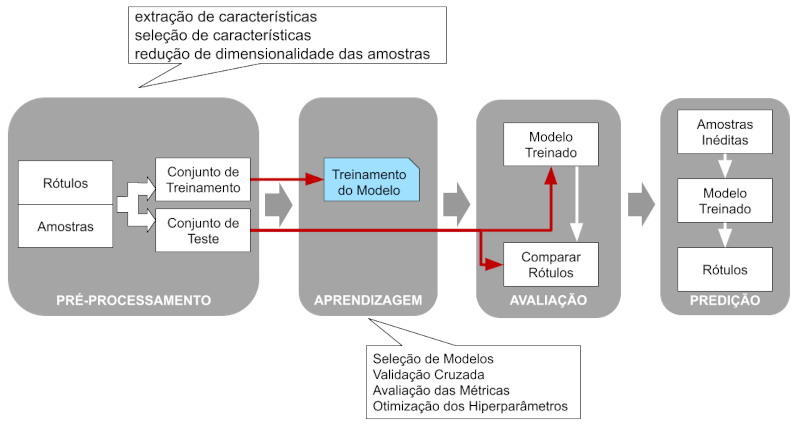
\includegraphics[width=\textwidth]{FIGURES/fig_6.png}
    \caption{Fases da vida de um modelo de aprendizado de máquina supervisionado. Fonte: Elaborada pelo autor com base em \citet{bib:livroRaschka}.}
    \label{fig:6}
\end{figure}

\begin{enumerate}[(i)]
    \item pré-processamento de dados;

    \item aprendizado;

    \item validação dos resultados;

    \item predição.
\end{enumerate}

É na primeira fase em que ocorre a extração dos dados brutos e a preparação destes para serem processados pelo algoritmo de ML. Esses dados dificilmente oferecem algum tipo de informação útil para que um modelo consiga gerar conhecimento; é necessário lapidá-los de forma a possibilitar que informações padronizadas sejam extraídas deles. Por essa razão, esta fase tende a ser uma das mais custosas de todo o ciclo de vida do uso de um modelo de aprendizado de máquina. Após a finalização da organização dos dados é que poderemos dividi-los em subconjuntos úteis para as demais fases: 

\begin{enumerate}[(a)]
    \item dados de treinamento;

    \item dados de teste;

    \item dados de validação.
\end{enumerate}

O primeiro subconjunto de dados é particularmente importante, pois é com ele que alimentamos o treinamento do modelo de aprendizado de máquina (fase (ii) do ciclo de vida). Neste conjunto, constam todos os dados válidos para treinamento (denominados atributos) e a respectiva resposta esperada para esses dados (também denominado rótulo). O segundo subconjunto é utilizado para verificar o quanto o modelo aprendeu com os dados de treinamento (fase (iii) do ciclo de vida). Basicamente, expõe-se o modelo aos dados de entrada inéditos e comparam-se os resultados de saída com os esperados para aqueles conjuntos de dados de entrada, possibilitando que se calcule a confiabilidade do modelo. É particularmente importante que os dados de treinamento e de teste sejam diferentes, afinal estamos utilizando um modelo de aprendizado de máquina para solucionar problemas desconhecidos, e não para explorar o que ele já conhece. Outro subconjunto de dados que pode ser utilizado é o de validação. Este é essencialmente similar ao subconjunto de dados de testes, só que com uma menor quantidade de dados, usados principalmente para verificar e ajustar os hiperparâmetros do modelo (explicaremos nos próximos parágrafos), quando necessário. O subconjunto de dados de validação é empregado interativamente com o conjunto de dados de treinamento, ainda na fase (ii) do ciclo de vida. Por fim, a fase (iv) do ciclo de vida é, em essência, a aplicação do modelo a situações reais, nas quais não há conhecimento prévio das saídas esperadas.

Há diversos algoritmos de aprendizado de máquina, classificados de acordo com sua forma de aprendizado \cite{bib:livroML} \cite{bib:livroKubat}. No \textbf{Aprendizado Supervisionado}, o resultado esperado (seja um dado categórico, seja um dado numérico) é conhecido e faz parte do conjunto de dados utilizados no processo de treinamento, conforme exemplos de dados apresentados anteriormente. Por outro lado, quando não há um resultado esperado ou quando este não é conhecido previamente ao processo de treinamento, empregam-se os modelos de \textbf{Aprendizado Não-Supervisionado}, cujo objetivo principal consiste justamente em encontrar as categorias ou valores que definem os dados de entrada, sendo especialmente útil para quando o objetivo do modelo é explorar os dados a fim de descobrir informações não óbvias. Por fim, há os modelos de \textbf{Aprendizado por Reforço}, em que o algoritmo aprende com os dados e se ajusta reiteradamente, utilizando mecanismos para atribuir penalidades (de modo a minimizar o erro) e recompensas (de modo a maximizar os acertos) ao longo das interações; isso possibilita que o modelo seja capaz de tomar decisões cada vez melhores, dentro de um ambiente dinâmico.

Sendo assim, quando observamos as classificações de aprendizado de máquina, conforme sua forma de aprendizado, e uma possível aplicação desses modelos em codificadores de vídeo, intuitivamente supomos que os modelos de aprendizado supervisionado sejam utilizados, uma vez que as decisões que podem ser tomadas já são conhecidas. Ou seja, apesar da elevada complexidade de um codificador de vídeo, as diversas etapas que o compõem possuem um rol limitado de opções de escolha; logo, modelos de aprendizado supervisionado são os mais adequados a esse contexto. Isso não significa que os demais algoritmos de aprendizado de máquina não possam ser aplicados a codificadores de vídeo, apenas que é menos comum.

Por fim, cabe definir o termo hiperparâmetro, que será utilizado nas próximas seções. Os hiperparâmetros são utilizados para configurar o funcionamento de algoritmos de aprendizado de máquina, tornando possível a geração de diferentes modelos preditivos com os mesmos dados de entrada. Cada algoritmo de aprendizado de máquina possui um conjunto de hiperparâmetros que podem ser configurados, como, por exemplo,a profundidade máxima das árvores treinadas em algoritmos do tipo árvore de decisão. Existe um grande número de hiperparâmetros que podem ser configurados em cada algoritmo e cada conjunto de configurações de hiperparâmetros é denominado combinação de hiperparâmetros. Alguns autores denominam essa combinação de hiperparâmetros como combinação candidata. Esta será também a nomenclatura adotada nas seções desta tese que tratam de soluções baseadas em aprendizado de máquina supervisionado.

\subsection{Aprendizado de Máquina Supervisionado}
\label{cap:2.3}

Como foi possível observar no início do capítulo \ref{cap:2}, a execução de um codificador de vídeo requer um elevado custo computacional, principalmente quando se utilizam codificadores baseados em formatos ou padrões mais atuais. Em parte, isso se relaciona com o aumento da complexidade das técnicas implementadas para realizar as predições e as compressões de dados. Uma das formas implementadas para reduzir o custo computacional é por meio do uso de algoritmos de aprendizado de máquina para acelerar tomadas de decisão do codificador. Dessa maneira, também se espera que o mesmo aconteça quando se utilizam transcodificadores de vídeo em que o conjunto de dados presentes durante o fluxo de execução do transcodificador pode ser reaproveitado pelos algoritmos de aprendizado de máquina. Como ficou mais claro na seção \ref{cap:2.2}, na área de codificação de vídeo, usam-se principalmente (mas não exclusivamente) os algoritmos de aprendizado supervisionado, já que é possível estruturar o conjunto de dados de treinamento em concordância com o rótulo de saída esperado.

Importante ressaltar que os rótulos de saída já são conhecidos, pois é possível executar o processo de codificação ou de transcodificação original de modo a se obter os valores durante e após a sua execução, o que justifica a maior presença dessa categoria de aprendizado de máquina nos trabalhos existentes na literatura científica. Como será explorado com mais detalhes no capítulo \ref{cap:3}, os algoritmos de aprendizado de máquina mais utilizados nos trabalhos de transcodificação de vídeo se baseiam em um dos três principais conceitos: árvores de decisão, classificadores lineares ou aprendizagem profunda.

O conceito de aprendizado de máquina baseado em árvore de decisão engloba algoritmos que geram uma estrutura de sequência de condicionais que parte do teste principal (com o atributo de maior relevância) até as respostas finais (folhas da árvore). Em razão disso, é facilmente implementável, tanto em software como em hardware, pois o treinamento e a execução do modelo não apresentam dificuldades. Podemos encontrar alguns algoritmos baseados em árvore de decisão, sendo que os mais comuns são o C4.5 \cite{bib:quinlan_2014}, o C5.0 \cite{bib:quinlan_2020} e o \textit{Random Forest} \cite{bib:breiman_2001}, além da versão de código aberto do C4.5, o J48.

Já os modelos baseados em classificador linear não são tão simples de ser treinados, pois se espera que os dados estejam, de alguma forma, agrupados em subconjuntos. Os algoritmos dessa classe tentam gerar uma equação algébrica capaz de separar um universo de N planos em regiões, no qual cada região corresponde a uma resposta final. Sendo assim, os modelos gerados a partir deles são mais difíceis de serem implementados. Contudo, \citet{bib:livroKubat} afirma que esse conceito de aprendizado de máquina é mais adequado para ser utilizado em conjuntos de dados com atributos mutuamente independentes. Fazem parte desse conceito os algoritmos \textit{Linear Discriminant Function} (LDF) \cite{bib:shumway_1974}, \textit{Support Vector Machine} (SVM) \cite{bib:hearst_1998} e o classificador linear \textit{Naïve-Bayes} \cite{bib:lewis_1998}.

Por fim, podemos encontrar entre os trabalhos de transcodificação de vídeo o uso de modelos de aprendizagem profunda (do inglês, \textit{Deep Learning}), cujo diferencial é a exigência de um grande número de dados para treinamento, o que eleva consideravelmente o custo computacional para utilizá-lo e exige um espaço de armazenamento alto. Apesar da probabilidade de acerto desses algoritmos serem muito interessantes, seu uso torna-se difícil em ambientes de restrição energética ou em soluções implementadas em hardware. Como veremos no capítulo \ref{cap:3}, na literatura científica em transcodificação de vídeo, poderemos encontrar soluções que empregam os algoritmos \textit{Convolutional Neural Network} (CNN) \cite{bib:koushik_2016} e \textit{Long Short-Term Memory} (LSTM) \cite{bib:graves_2012}.

Diante de tantas opções de conceitos e algoritmos de aprendizado de máquina, o número de possíveis modelos treinados para solucionar um mesmo problema é exponencial, já que cada nova possibilidade é um fator multiplicador a todas as combinações já consideradas. Por consequência, é preciso saber quais deles são mais ou menos apropriados para resolver determinados problemas. Para possibilitar a averiguação da viabilidade desses modelos, temos que mensurar a confiabilidade de cada um deles, conforme veremos na próxima seção.

\section{Confiabilidade dos Modelos de Aprendizado de Máquina}
\label{cap:2.4}

Inserir um conjunto específico de dados na entrada de um modelo de aprendizado de máquina, capturar sua resposta e compará-la com a resposta esperada é a forma mais simples de verificação da exatidão da resposta desse modelo. No entanto, um único caso de teste não é estatisticamente válido, por isso, utilizam-se diversos casos, preferencialmente diferentes dos utilizados para treinamento. A média de acertos ($\mu$), definida pela Equação \ref{eq:1}, é pouco empregada de forma isolada na literatura científica, pois não informa muito sobre que tipos de acertos e erros foram performados.

\begin{equation}
    \label{eq:1}
    \mu = \frac{acertos}{total}
\end{equation}

Aqui é importante definir que os modelos de aprendizado de máquina podem retornar respostas complexas. Contudo, para facilitar as explicações desta seção, consideramos modelos cujas respostas sejam valores binários. Inclusive, essa é a forma mais comum de respostas que se observam nos trabalhos com codificação de vídeo. Assim exposto, são esperados quatro tipos de respostas de qualquer modelo com decisões binárias: 

\begin{enumerate}[a)]
    \item \textbf{Verdadeiros Positivos} (VP), ou seja, o modelo retorna positivo quando a resposta de fato é positiva;
    
    \item \textbf{Verdadeiros Negativos} (VN), ou seja, o modelo retorna negativo quando a resposta de fato é negativa;
    
    \item \textbf{Falso Negativo} (FN), quando o modelo retorna negativo quando deveria ter retornado positivo;
    
    \item \textbf{Falso Positivo} (FP), quando o modelo retorna positivo quando deveria ter retornado negativo.
\end{enumerate}

É importante ressaltar que, em modelos cuja decisão possue um rótulo não-binário, esses quatro tipos de resposta ainda estão presentes, mas distribuídos em $2^{rotulos}$ subtipos. Nesta tese, não abordamos avaliações dessa complexidade, mas as referências para tal estão disponíveis em \citet{bib:livroKubat}, \citet{bib:livroML} e \citet{bib:livroRaschka}. Segundo essas referências, as quatro respostas de um modelo binário resultam na matriz de confusão (do inglês, \textit{confusion matrix}), representada na Tabela \ref{tab:II}, na qual, na diagonal, estão as respostas corretas e, nas demais células, estão as respostas erradas.

\begin{table}
\begin{center}
\caption{Matriz de confusão das respostas de um modelo de aprendizado de máquina.}
\label{tab:II}
\footnotesize

\begin{tblr}{
    colspec = {c|c|c|c},
    hlines,
    row{even} = {gray9}
}
\hline
\SetCell[c=2,r=2]{}&& \SetCell[c=2]{c}\textbf{Rótulos Preditos} \\
&& \textbf{Positivo} & \textbf{Negativo} \\
\SetCell[r=2]{c}\textbf{Rótulos Esperados} & \textbf{Positivo} & VP & FN \\
 & \textbf{Negativo} & FP & VN \\
\hline
\end{tblr}
\end{center}
\end{table}


Com essa matriz de confusão, é possível estabelecer o desbalanceamento da predição feita pelo modelo. É esperado que, na diagonal, os valores sejam elevados. No entanto, saber se o modelo tende a errar mais em falsos positivos ou falsos negativos pode ajudar o pesquisador a definir melhorias ou identificar relações ocultas entre as respostas preditas e esperadas. E não apenas isso: também pode ajudá-lo a identificar se o modelo treinado de fato é apto para ser utilizado em um determinado contexto. Por exemplo, no caso de um modelo em treinamento para identificar a contaminação de paciente por COVID-19, um elevado número de falsos negativos em relação a falsos positivos seria péssimo, pois pessoas infectadas poderiam ser liberadas ao convívio social, acarretando um grave problema de saúde pública. Um segundo exemplo, em que os valores de falso positivo sejam maiores que os falsos negativos, pode ser particularmente ruim caso o modelo esteja sendo utilizado para identificar a venda de ações na bolsa de valores. Nota-se que, apesar de os tipos de rótulos serem os mesmos, o contexto em que estão inseridos é de extrema importância. Demonstramos, assim, que definir e avaliar a confiabilidade do modelo não é tarefa trivial.

Por essa razão, existem diversas métricas baseadas nessa matriz de confusão, cada uma mais adequada para identificar características específicas ao contexto desejado. São elas:

\textbf{Nível de Acurácia} (do inglês, \textit{Accuracy}): Em essência, é a média apresentada na Equação \ref{eq:1}. O nível de acurácia apresenta uma relação entre as respostas corretas e todas as respostas que o modelo prediz. No contexto da matriz de confusão, a acurácia é calculada conforme a Equação \ref{eq:2}:

\begin{equation}
    \label{eq:2}
    accuracy = \frac{VN+VP}{VN+VP+FN+FP}
\end{equation}

\textbf{Nível de Precisão} (do inglês, \textit{Precision}): Informa quantas respostas corretas o modelo apresentou, considerando apenas as classificadas como verdadeiras. Essa métrica é principalmente útil quando o número de FP é mais prejudicial que o número de FN, vide exemplo da bolsa de valores mencionado anteriormente. A precisão pode ser calculada conforme a Equação \ref{eq:3}:

\begin{equation}
    \label{eq:3}
    precision = \frac{VP}{VP+FP}
\end{equation}

\textbf{Nível de Sensibilidade} (do inglês, \textit{Sensitivity}): Informa quantos rótulos existentes são verdadeiramente positivos. É uma métrica particularmente útil para identificar o quão bom um modelo treinado poderá ser em detectar respostas corretas. A sensibilidade poderá ser calculada conforme a Equação \ref{eq:4}:

\begin{equation}
    \label{eq:4}
    sensitivity = \frac{VP}{VP+FN}
\end{equation}

\textbf{Nível de Especificidade} (do inglês, \textit{Recall}): Enquanto o nível de sensibilidade informa sobre os casos positivos, o nível de especificidade informa o quão bom o modelo poderá ser em identificar os verdadeiros casos negativos. A especificidade pode ser calculada conforme a Equação \ref{eq:5}:

\begin{equation}
    \label{eq:5}
    recall = \frac{VN}{VN+FP}
\end{equation}

\textbf{Pontuação F1} (do inglês, \textit{F1-Score}): Se as métricas de precisão e sensibilidade informam, cada uma, o quão bom o modelo poderá ser em identificar casos verdadeiramente positivos e negativos, respectivamente, a métrica F1 unifica as duas métricas anteriores em um só valor. Dessa forma, facilita a relação geral do modelo em realizar boas predições binárias. O F1 poderá ser calculado por meio da média harmônica apresentada na Equação \ref{eq:6}:

\begin{equation}
    \label{eq:6}
    f1 = 2*\frac{precision*sensitivity}{precision+sensitivity}
\end{equation}

\textbf{Área sob a Curva ROC} (do inglês, \textit{Area Under the Curve}, AUC): Existe um gráfico denominado Características Operacionais do Receptor (do inglês, \textit{Receiver Operating Characteristics}, ROC), que apresenta, de forma gráfica (linha azul da Figura \ref{fig:8}), o desempenho de um modelo em classificar dados binários. Para tanto, relaciona as probabilidades da sensibilidade e o inverso da especificidade, ou seja, a relação entre os verdadeiros positivos e os falsos positivos. Assim, é possível extrair a área sob a curva ROC (área amarela da Figura \ref{fig:8}), por meio de um cálculo integral, e representar numericamente a relação apresentada no gráfico. A métrica AUC apresenta uma estimativa de desempenho de classificação do modelo ao considerar as taxas que o modelo prediz como verdadeiras e os valores reais desses rótulos. Em outras palavras, a AUC informa a probabilidade de o modelo retornar uma resposta positiva corretamente. Lembrando que ROC considera apenas valores binários, respostas aleatórias (reta laranja da Figura \ref{fig:8}) retornam 0,5 e um modelo capaz de acertar todas as respostas retorna 1,0. Portanto, a AUC informa algum valor entre esses dois limites, já que AUC inferior a 0,5 indica um péssimo modelo preditivo. A métrica AUC é especialmente útil para comparar modelos diferentes.

\begin{figure}
    \centering
    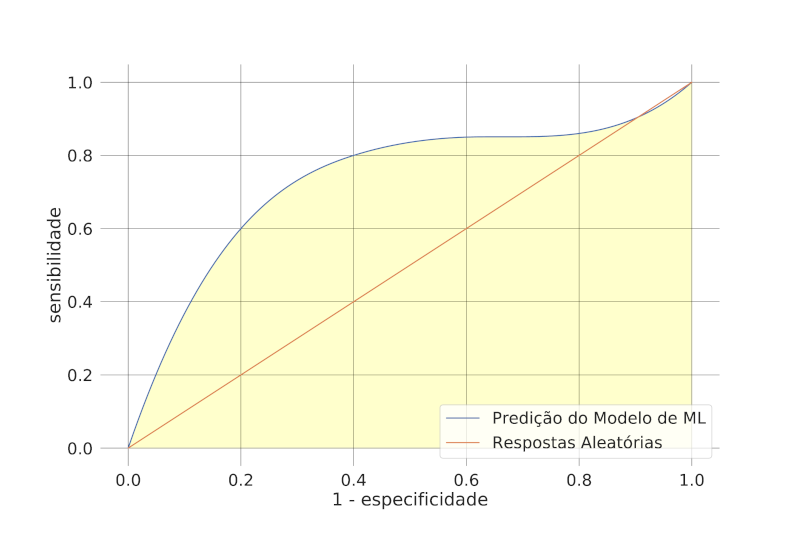
\includegraphics[width=0.85\textwidth]{FIGURES/fig_8.png}
    \caption{Exemplo da curva ROC e AUC (destacada em amarelo). Fonte: Elaborada pelo autor.}
    \label{fig:8}
\end{figure}

Outras métricas estatísticas também podem ser utilizadas, tais como t-\textit{Student} ou valor-\textit{p}, conforme \citet{bib:livroML} e \citet{bib:livroKubat}. Todavia, com menor probabilidade de uso. Dessa forma, apenas as métricas apresentadas acima são consideradas ao longo desta tese e, em particular, as métricas \textit{F1-Score} e AUC, por apresentarem maior confiabilidade nos resultados verdadeiramente válidos.

\section{Comparando Codificações}
\label{cap:2.5}

Para finalizar este capítulo, é de especial interesse abordar a forma como é feita a comparação entre duas codificações de vídeo diferentes. De forma geral, três valores são capturados durante uma codificação de vídeo: 

\textbf{Taxa de bits por segundo} (do inglês, \textit{bits per second}, bps): representa quantos bits ou kilobits (kb) o \textit{bitstream} gerado possui divididos pelo tempo em segundos do vídeo. Como esse valor é relativo à quantidade de quadros processados, a maioria dos codificadores já fornece esse valor médio.

\textbf{Nível da qualidade da imagem}: indica a diferença objetiva entre a imagem original (pré-codificada) e a imagem decodificada (pós-codificada). Existe, na literatura, uma série de métricas objetivas que capturam a diferença entre as duas imagens, sendo as mais comuns a Relação Sinal-Ruído de Pico (do inglês, \textit{Peak Signal-to-Noise Ratio}, PSNR) \cite{bib:psnr} e a Fusão de Vários Métodos de Avaliação de Vídeo (do inglês, \textit{Video Multi-Method Assessment Fusion}, VMAF) \cite{bib:vmaf}. O valor da métrica PSNR, assim como a taxa de bits, já é fornecido pela maioria dos codificadores após a codificação. Portanto, é a mais usual de ser encontrada na literatura científica, apesar das diversas inconsistências que essa métrica oferece quando comparada com métricas subjetivas ou empregada em vídeos mais complexos, como HDR ou \textit{Screen Content} \cite{bib:mse_wrong}. Note que o cálculo do PSNR é sempre resultante da diferença entre a sequência de vídeo original (âncora) com a versão dessa sequência após a codificação (comparada). Além disso, na transcodificação de vídeos, o PSNR é calculado tendo-se a sequência decodificada como âncora e a sequência re-codificada como comparada.

\textbf{Variação do Tempo de Codificação}: informa a diferença percentual entre o tempo exigido para executar a codificação em observação e o tempo de codificação de referência. Os trabalhos de transcodificação de vídeo apresentados nesta tese visam sempre apresentar um tempo de codificação inferior ao de referência. Portanto, normalmente se apresentam valores de Redução de Tempo (do inglês, \textit{Time Saving}, TS). Para o cálculo da redução do tempo de codificação ou de transcodificação, utilizamos a Equação \ref{eq:7}, onde $Ta$ e $Tb$ são os tempos de codificação original e modificada, respectivamente, e $q$ representa o conjunto de níveis de quantização utilizados.

\begin{equation}
    \label{eq:7}
    TS = 100 * \left ( \frac{1}{n} \sum_{q_0}^{q_n} \frac{Ta_q - Tb_q}{Ta_q} \right )
\end{equation}

É importante destacar que existe uma relação entre a taxa de bits por segundo e o nível da qualidade da imagem, isto é, uma maior quantidade de dados permite armazenar vídeos com maior qualidade de imagem. Ao mesmo tempo, codificadores de vídeo mais modernos são capazes de comprimir vídeos com idêntico nível de qualidade de imagem que outro codificador mais antigo, mas com uma quantidade inferior de dados. Portanto, essa relação entre taxa de bits e qualidade de imagem precisa ser considerada ao se realizar comparações entre diferentes codificadores ou variações de um mesmo codificador. O principal destaque a ser feito é que os níveis de qualidade da imagem também são alterados, o que dificulta a correlação direta nessas comparações.

Dessa forma, \citet{bib:bdrate} desenvolveu uma métrica, denominada Bj{\o}ntegaard Delta(BD)-rate, que relaciona duas codificações diferentes sob a ótica dessas duas variáveis alvo. Para tanto, faz uso do cálculo de uma integral que representa a área entre duas curvas de taxa de bits e nível de qualidade, como apresentado na Figura \ref{fig:9}. Basicamente, o BD-rate equipara os níveis de qualidade e informa a diferença percentual da taxa de bits de uma codificação em relação à codificação de referência. Sendo assim, valores negativos indicam uma redução na taxa de bits, o que é normalmente esperado quando se comparam formatos de codificação de vídeo recentes frente aos mais antigos. Por outro lado, valores positivos de BD-rate indicam um aumento na taxa de bits, o que é mais comum ocorrer nos trabalhos de transcodificação de vídeo acelerado frente aos transcodificadores originais.

\begin{figure}
    \centering
    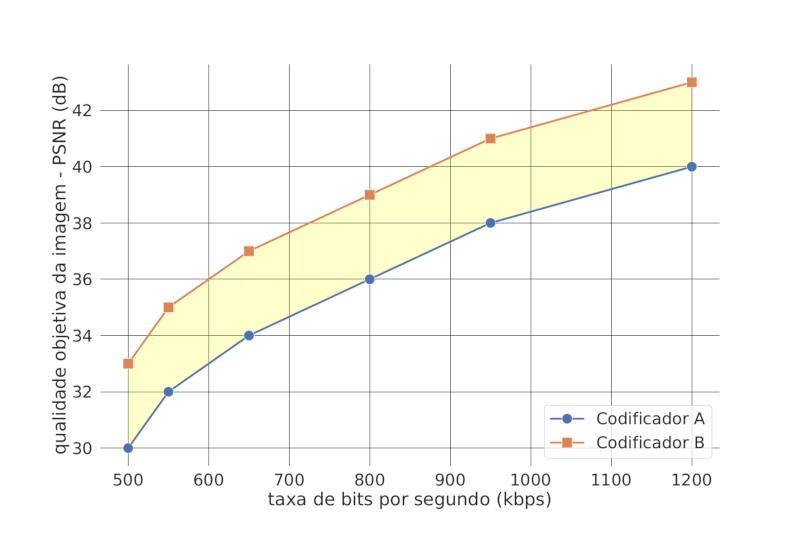
\includegraphics[width=0.85\textwidth]{FIGURES/fig_9.png}
    \caption{Exemplificando duas curvas de BD-rate. Fonte: Elaborada pelo autor.}
    \label{fig:9}
\end{figure}

Finalizamos, então, todos os conceitos básicos necessários para a compreensão do restante desta tese. Para conhecimentos mais aprofundados, recomendamos a leitura das referências bibliográficas apontadas ao longo deste capítulo. No capítulo \ref{cap:3}, apresentamos o estado da arte em transcodificação de vídeo.

